%to have line numbers
%\RequirePackage{lineno}
\documentclass[10pt, letterpaper]{article}      
\usepackage[margin=.1cm,font=small,labelfont=bf]{caption}[2007/03/09]
%\usepackage{endnotes}
%\let\footnote=\endnote
\usepackage{setspace}
\usepackage{longtable}                        
\usepackage{anysize}                          
\usepackage{natbib}                           
%\bibpunct{(}{)}{,}{a}{,}{,}                   
\bibpunct{(}{)}{,}{a}{}{,}                   
\usepackage{amsmath}
\usepackage[% draft,
pdftex]{graphicx} %draft is a way to exclude figures                
\usepackage{epstopdf}
\usepackage{hyperref}                             % For creating hyperlinks in cross references
\hypersetup{pdfborder={0 0 0.4}} %have nice light boxes on refs

% \usepackage[margins]{trackchanges}

% \note[editor]{The note}
% \annote[editor]{Text to annotate}{The note}
%    \add[editor]{Text to add}
% \remove[editor]{Text to remove}
% \change[editor]{Text to remove}{Text to add}

%TODO make it more standard before submission: \marginsize{2cm}{2cm}{1cm}{1cm}
\marginsize{1cm}{1cm}{.5cm}{.5cm}%{left}{right}{top}{bottom}   
					          % Helps LaTeX put figures where YOU want
 \renewcommand{\topfraction}{1}	                  % 90% of page top can be a float
 \renewcommand{\bottomfraction}{1}	          % 90% of page bottom can be a float
 \renewcommand{\textfraction}{0.0}	          % only 10% of page must to be text

 \usepackage{float}                               %latex will not complain to include float after float

\usepackage[table]{xcolor}                        %for table shading
\definecolor{gray90}{gray}{0.90}
\definecolor{orange}{RGB}{255,128,0}

\renewcommand\arraystretch{.9}                    %for spacing of arrays like tabular

%-------------------- my commands -----------------------------------------
\newenvironment{ig}[1]{
\begin{center}
 %\includegraphics[height=5.0in]{#1} 
 \includegraphics[height=3.3in]{#1} 
\end{center}}

 \newcommand{\cc}[1]{
\hspace{-.13in}$\bullet$\marginpar{\begin{spacing}{.6}\begin{footnotesize}\color{blue}{#1}\end{footnotesize}\end{spacing}}
\hspace{-.13in} }

%-------------------- END my commands -----------------------------------------



%-------------------- extra options -----------------------------------------

%%%%%%%%%%%%%
% footnotes %
%%%%%%%%%%%%%

%\long\def\symbolfootnote[#1]#2{\begingroup% %these can be used to make footnote  nonnumeric asterick, dagger etc
%\def\thefootnote{\fnsymbol{footnote}}\footnote[#1]{#2}\endgroup}	%see: http://help-csli.stanford.edu/tex/latex-footnotes.shtml

%%%%%%%%%%%
% spacing %
%%%%%%%%%%%

% \abovecaptionskip: space above caption
% \belowcaptionskip: space below caption
%\oddsidemargin 0cm
%\evensidemargin 0cm

%%%%%%%%%
% style %
%%%%%%%%%

%\pagestyle{myheadings}         % Option to put page headers
                               % Needed \documentclass[a4paper,twoside]{article}
%\markboth{{\small\it Politics and Life Satisfaction }}
%{{\small\it Adam Okulicz-Kozaryn} }

%\headsep 1.5cm
% \pagestyle{empty}			% no page numbers
% \parindent  15.mm			% indent paragraph by this much
% \parskip     2.mm			% space between paragraphs
% \mathindent 20.mm			% indent math equations by this much

%%%%%%%%%%%%%%%%%%
% extra packages %
%%%%%%%%%%%%%%%%%%

\usepackage{datetime}


\usepackage[latin1]{inputenc}
\usepackage{tikz}
\usetikzlibrary{shapes,arrows,backgrounds}


%\usepackage{color}					% For creating coloured text and background
%\usepackage{float}
\usepackage{subfig}                                     % for combined figures

\renewcommand{\ss}[1]{{\colorbox{blue}{\bf \color{white}{#1}}}}
\newcommand{\ee}[1]{\endnote{\vspace{-.10in}\begin{spacing}{1.0}{\normalsize #1}\end{spacing}\vspace{.20in}}}
\newcommand{\emd}[1]{\ExecuteMetaData[/tmp/tex]{#1}} % grab numbers  from stata

%TODO before submitting comment this out to get 'regular fornt'
\usepackage{sectsty}
\allsectionsfont{\normalfont\sffamily}
\usepackage{sectsty}
\allsectionsfont{\normalfont\sffamily}
\renewcommand\familydefault{\sfdefault}

%\usepackage[margins]{trackchanges}
\usepackage{rotating}
\usepackage{catchfilebetweentags}

\usepackage{abstract}
\renewcommand{\abstractname}{}    % clear the title
\renewcommand{\absnamepos}{empty} % originally center
%-------------------- END extra options -----------------------------------------
\date{{}\today \hspace{.2in}\xxivtime}
\title{  % remember to have Vistula University!!
  Hey! Cities! Leave Them Kids Alone! \\ \Large{(Adolescents Are Less Happy in Cities)} %(urban unhappiness is common in adolescents)
}
\author{
% Adam Okulicz-Kozaryn\thanks{EMAIL: adam.okulicz.kozaryn@gmail.com
%   \hfill I thank XXX.  All mistakes are mine.} \\
% {\small Rutgers - Camden  % and Vistula University
% }
}

\begin{document}

%%\setpagewiselinenumbers
%\modulolinenumbers[1]
%\linenumbers

\bibliographystyle{/home/aok/papers/root/tex/ecta}
\maketitle
\vspace{-.4in}
\begin{center}

\end{center}


\begin{abstract}
\noindent strong effects! on the whole, 0.5 on 1-10 scale, and for some countries close to 1!
\end{abstract}
\vspace{.15in} 
\noindent{\sc %XXX TODO add to ebib as keyword PAPER-CODE-NAME and tag with ebib keywords 
} 
\vspace{.25in} 

\begin{spacing}{1.4} %TODO MAYBE before submission can make it like 2.0
\rowcolors{1}{white}{gray90}

%  instead \ExecuteMetaData[../out/tex]{ginipov} do \emd{ginipov}

% \begin{figure}[H]
%  \includegraphics[height=3in]{../out/gov_res_trust.pdf}\centering\label{gov_res_trust}
% \caption{woo}
% \end{figure}


%TODO !!!! have input here aok_var_des

We know that adults tend to be less happy in cities across the world (except in
the poorest nations such as Sub-Saharan Africa) \citep{aok21}. But we do not
know about the children. 

\section{theory and mechanisms of urban unhappiness}

% rephraze copied from swbUrbRurPsid
 Genes determine about half of SWB
 \citep{schnittker08,lykken96t,brooksGenetic}.
 %
 Humans have not
evolved for city life among thousands of people densely packed together in an
artificial setting, i.e., in a city. For over 95\% of human evolutionary history there were no cities--hunters-gatherers lived in bands of 50-80 \citep{maryanski92}. 
%Humans have evolved to prefer and be happy in nature,  open space
%there was that citation that i have recently seen but forgot where that that
%humans evolved to prefer nature--those who prefered it and were in harmony with
%it were more likely to survive etc


Ingroup preference or homophily (``love of the same'') theory
  states
that a  human has a preference for other humans like her \citep{mcpherson01,tajfel82,tajfel71,smelser99,putnam07,christakis09f}. % , and outgroups contain dissimilar persons.
 A defining
feature of a city is heterogeneity or diversity \citep{wirth38}, which
accordingly produces: 
 mistrust, uneasiness, conflict, and misanthropy
 \citep{milgram70,thrift05,amin06}.\footnote{
 Yet, on the other hand, in a city there can be community, a neighborhood
village, that at least in some ways can simulate a more natural habitat for a
human \citep{fischer95,fischer75,jacobs93}.}

Livability theory \citep{veenhoven95,veenhoven14b,veenhoven00b} states that
humans, just as other animals, have needs (such as those on Maslow hierarchy of
needs \citep{maslow87}), and if those needs are satisfied, then conditions are
livable and happiness follows. As opposed to evolution and homophily
predicting urban unhappiness, it is unclear what livability theory
 predicts regarding urbanism. Some aspects of urbanism may
 improve livability, and hence, happiness.
  %
 Cities have multiple benefits  \citep{meyer13,florida08,glaeser11,osullivan09}, notably jobs and amenities that improve livability and
 happiness. But cities also do have multiple disamenities such as more congestion, crime,
   infectious  disease spread, air, noise, and light pollutions
   \citep{bettencourt10b,bettencourt07,meyer13,aokCityBook15}.\footnote{Measuring
     it with happiness yardstick,  city disadvantages outweigh city
     advantages--cities are less happy (at least in the developed world)
     \citep{aok21}.} 
 %
   And those disamenities may especially affect adolescents. Urban
 crime (and bullying) is perhaps more of a problem for adolescents (especially
 females) than for adults who may be better able to insulate themselves from
 it\footnote{An adult would spend much time at work, home, or in a
   car, which are relatively crime free. An adolescent is arguably less able to
   insulate herself from neighborhood and peers, which are often infested with
   crime in large cities. It needs to be remebered that crime is a a city
   feature--all large cities have large crime problem--crime  does increase
   extremely consistently with city size \cite{blissCL_nov4_14,bettencourt13,bettencourt10,bettencourt10b,bettencourt07}.}
 and cope with it. Clearly, by definition, adults have better coping mechanisms
 than more fragile adolescents. 

 It has been theoretized already a century ago that urbanism has a negative
 effect on human brains / neural processing \citep{simmel03}, and it has been
 recently confirmed by neuroscience including that even growing up in a city has
 lasting negative effects later in life \citep{lederbogen11}. Again adolescents
 are more at risk than adults. 
   
   Multiple Discrepancies Theory (MDT) \citep{michalos85,michalos14c} states that
happiness is relative and a result of multiple comparisons. Arguably, visual and social comparisons are more likely in
urban areas as there are more people and more stimuli. And there is some
evidence that humans tend to make upwards comparisons \citep{frey02s} thus
ending up relatively deprived \citep[e.g.,][]{luttmer05,frank12}.

Adolescents, like adults, are likely to want to keep up with Joneses, but in
slightly different ways, e.g., clothing, jewelry, parties, cars--see some
examples in \citet{frank12}.

Finally a big, maybe the biggest, happiness killer of the youth is social media
\cite{twengeATL17sep,twenge14}.


\section{Happiness in Kids}

TODO: write sth about happness in kids; btw looks like they used normal happiness question; not smileys


\section{Data}

We use 2018 pisa from \url{https://www.oecd.org/pisa/data/2018database/}. Age is 15 to 16.3, so not kids kids but more like
little adolescents.

Urbanicity is recorded in  School questionnaire administered to school
principals:

Which of the following definitions best describes the community in which your school is located?
\begin{itemize}
\item A village, hamlet or ruralarea (fewer than 3 000 people)
\item A small town (3 000 to about 15 000 people)
\item A town (15 000 to about 100 000 people)
\item A city (100000 to about 1 000 000 people)
\item A large city (with over 1 000 000 people)
\end{itemize}

A nice feature of PISA data is that there are large cities, lt1m, in wvs for
instacne the top bin is only 500k. And it is missing for only 6 percent of
observations. 

a limitation is that we do not see a good health variable--exisiting ones are
missing for vast majroity. Health is of course a key happiness predictor, but
arguably less imoportant for kids as they are healthier than adults. 


PISA 2018 defines meaning in life as the extent to which 15-year-olds
comprehend, make sense of, or find significance in their lives
\citep{pisa18}. PISA 2018 asked students whether they agree or disagree (
"strongly disagree", "disagree", "agree", "strongly agree") with the following
statements: "My life has clear meaning or purpose"; "I have discovered a
satisfactory meaning in life"; and "I have a clear sense of what gives meaning
to my life". These statements were combined to create the index of meaning in
life

We control for internet use, and we do  have specific measures how used, eg we
 measure social media use.  We also measure out of school usage and useage ``for
 fun''--see table \ref{var_des} for all variables definitions. 

\input{varDes.tex} 

\section{Results}

%meh have plenty of tables
% \begin{figure}[H]
%  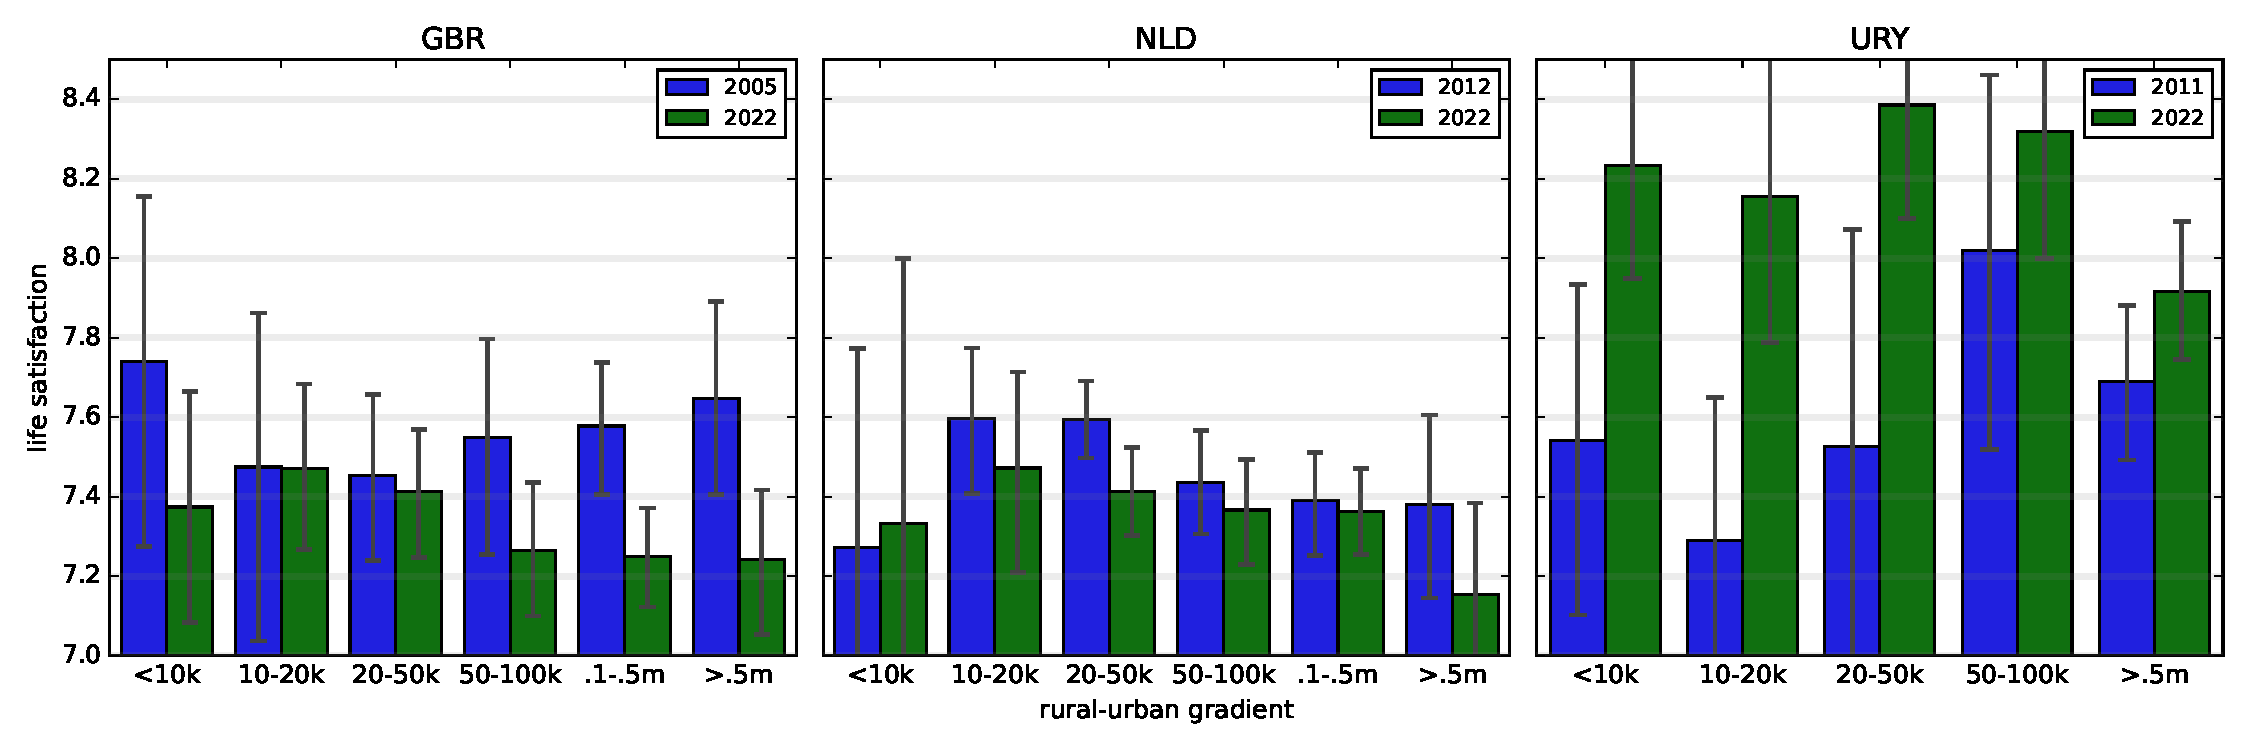
\includegraphics[height=3in]{bar.pdf}\centering\label{bar}
% \caption{Mean of life satisfaction and eudamonia by urbanicity.}
% \end{figure}


The differences are large--about .5 on 0-10 SWB scale. It needs to be remembered
that ecological variables have small effects on SWB as
 expected--most SWB is explained by genes \citep{schnittker08} and person level
 predictors \citep{veenhoven14b}). % . Still, the leading social scientists
 % such as Amartya Sen and Ed Diener advocate use of SWB for
 % public policy \citep{stiglitz09al,diener09}.
 %
 %
 %
 %
 And in a1-a3\footnote{Not
in a4 controling for country dummies.} there is a big
difference between the largest cities (gt1m) and everything else just as for
adults \citep{aok-ls_fisher16}. But interestingly, not necessarily like adults,
there is also a large gap between lt3k and 3-15k, again especially in models
a1-a3, perhaps in the open country there are best outdoor play opportunities for
the kids.

As in adults \citep{aok21}, addition of income/wealth makes results
stronger--income/wealth confounds with urbanicity.

In full model a4 results are strong, beta (fully standardized; not shown) for
gt1m is 65 percent of wealth.

Finally we split by gender in a4m and a4f--interestingly city penaly higher for
female; arguably because fem more affected by urban crime

And finally finally add the 4 internet use variables in a5 (we postpone it to
the last model as the internet variables cut the sample size by about 200k),
results are similar\footnote{Actually interent use has very low correlation
  with urbanicity--see online appendix for details. It probably has been the case
  that internet was more of an urban phenomenon, but in an era of
  smartphones--they are ubiquitious throught degrees of urbanness and
  development levels.}

\begin{table}[H]\centering\caption{OLS regressions of life satisfaction.} \label{regA} \begin{scriptsize} \begin{tabular}{p{2.2in}p{.6in}p{.6in}p{.6in}p{.6in}|p{.6in}p{.6in}|p{.6in}p{.6in}p{.6in}p{.6 in}p{.6in}p{.6 in}}\hline                     &   $<.5m$   &     $>.5m$   &   $<.5m$   &     $>.5m$   &   URYrurTow   &     URYcity   \\
2022                &       -0.21** &       -0.41** &       -0.12** &       -0.23   &        0.75***&        0.23+  \\
constant            &        7.54***&        7.65***&        7.50***&        7.38***&        7.54***&        7.69***\\
N                   &        3111   &         521   &        3572   &         373   &        1154   &         836   \\
 \hline\multicolumn{4}{l}{*p$<$0.05 **p$<$0.01 ***p$<$0.001} \end{tabular}\end{scriptsize}\end{table}




\begin{spacing}{.9} \begin{table}[H]\centering   \begin{scriptsize} \begin{tabular}{p{.5in}p{.5in}p{.5in}p{.5in}p{.5in}p{.5in}p{.5in}p{.5in}p{.5in}p{.5in}p{.5
                                                                      in}p{.5in}p{.5
                                                                      in}}\hline
                                                                      \input{../out/a4cou.tex}
                                                                      \hline *
                                                                      p$<$0.05,
                                                                      $+$
                                                                      p$<$0.1;
                                                                      robust std
                                                                      err \end{tabular}\end{scriptsize}\caption{\label{a4cou}OLS
                                                                    regressions
                                                                    of life satisfaction on
                                                                    place size
                                                                    for each
                                                                    country
                                                                    separately
                                                                    includiOBng
                                                                    covariates
                                                                    from a4 (not
                                                                    shown). Only
                                                                  LBN and HUN
                                                                  marginally
                                                                  happier in
                                                                  cities lt1m
                                                           }\end{table} \end{spacing}


\subsection{Eudamonia}

in table \ref{regB} different from lifests, biggest hit from lt3k to 3-15k in b1-b3, and in b4
controllig for countruy dummies rather smooth gradient. females aboy 2x less
eudamonia than males in urb v rural\\

And like with life satisfaction controling for internet use does not change lt1m coefficent significantly 

\begin{table}[H]\centering\caption{OLS regressions of Eudamonia.} \label{regB} \begin{scriptsize} \begin{tabular}{p{2.2in}p{.6in}p{.6in}p{.6in}p{.6in}|p{.6in}p{.6in}|p{.6in}p{.6in}p{.6in}p{.6 in}p{.6in}p{.6 in}}\hline                     &   $<.5m$   &     $>.5m$   &   $<.5m$   &     $>.5m$   &   URYrurTow   &     URYcity   \\
2022                &       -0.18*  &       -0.39+  &       -0.20***&       -0.45** &        0.42***&        0.21   \\
income              &        0.09***&        0.01   &        0.06***&        0.14***&        0.07*  &        0.13***\\
age                 &       -0.03*  &       -0.08** &       -0.02+  &       -0.06+  &        0.00   &       -0.06** \\
age2                &        0.00** &        0.00** &        0.00** &        0.00*  &       -0.00   &        0.00** \\
male                &       -0.18** &       -0.13   &       -0.11*  &       -0.27+  &        0.06   &        0.19   \\
married or living together as married&        0.53***&        0.74***&        0.44***&        0.23   &        0.46** &        0.06   \\
divorced/separated/widowed&        0.07   &        0.15   &       -0.11   &       -0.14   &       -0.37+  &       -0.19   \\
autonomy            &       -0.11*  &       -0.07   &       -0.11** &       -0.01   &       -0.06   &        0.06   \\
freedom             &        0.44***&        0.42***&        0.35***&        0.43***&        0.43***&        0.36***\\
trust               &        0.12+  &        0.42** &        0.43***&        0.28+  &       -0.05   &        0.10   \\
postmaterialist     &       -0.05   &       -0.18   &       -0.11*  &        0.14   &       -0.02   &        0.15   \\
god important       &        0.01   &        0.05*  &        0.02*  &       -0.01   &        0.05** &        0.06** \\
constant            &        4.08***&        5.95***&        4.59***&        4.80***&        3.47***&        4.58***\\
N                   &        1985   &         309   &        2283   &         237   &         736   &         579   \\
 \hline\multicolumn{4}{l}{*p$<$0.05 **p$<$0.01 ***p$<$0.001} \end{tabular}\end{scriptsize}\end{table}

in atble \ref{b4cou} urban eudamia penalty is less clear than life
satisfaction--while most countries do have urban penalty, there is a handful
with urban eudamonic premium


\begin{spacing}{.9} \begin{table}[H]\centering   \begin{scriptsize} \begin{tabular}{p{.5in}p{.5in}p{.5in}p{.5in}p{.5in}p{.5in}p{.5in}p{.5in}p{.5in}p{.5in}p{.5
                                                                      in}p{.5in}p{.5
                                                                      in}}\hline
                                                                      \input{../out/b4cou.tex}
                                                                      \hline *
                                                                      p$<$0.05,
                                                                      $+$
                                                                      p$<$0.1;
                                                                      robust std
                                                                      err \end{tabular}\end{scriptsize}\caption{\label{b4cou}OLS
                                                                    regressions
                                                                    of Eudamonia on
                                                                    place size
                                                                    for each
                                                                    country
                                                                    separately
                                                                    including
                                                                    covariates
                                                                    from b4 (not
                                                                    shown). Most
                                                                    countries
                                                                    eudamoinc
                                                                    urban
                                                                    penalty, but
                                                                    a
                                                                    handful of
                                                                    countries
                                                                    have premium
                                                           }\end{table} \end{spacing}




\section{Conclusion and discussion}

Future research:
Arguably after the pandemic cities became even more unhappy just as adults did
\textbf{??blind for peer-review}

                                                       
% %table centered on decimal points:)
% \begin{table}[H]\centering\footnotesize
% \caption{\label{freq_im_god} importance of God}
% \begin{tabular} {@{} lrrrr @{}}   \hline 
% Item& Number & Per cent   \\ \hline
% 1(not at all)&    9,285&  9\\
% 2&    3,555&        3\\
% 3&    3,937&        4\\
% 4&    2,888&        3\\
% 5&    7,519&        7\\
% 6&    5,175&        5\\
% 7&    6,050&        6\\
% 8&    8,067&        8\\
% 9&    8,463&        8\\
% 10&   52,385&       49\\
% Total&  107,324&      100\\ \hline
% \end{tabular}\end{table}


% % Define block styles
% \tikzstyle{block} = [rectangle, draw, fill=black!20, 
%     text width=10em, text centered, rounded corners, minimum height=4em]
% \tikzstyle{b} = [rectangle, draw,  
%     text width=6em, text centered, rounded corners, minimum height=4em]
% \tikzstyle{line} = [draw, -latex']
% \tikzstyle{cloud} = [draw, ellipse,fill=black!20, node distance = 5cm,
%     minimum height=2em]
    
% \begin{tikzpicture}[node distance = 2cm, auto]
%     % Place nodes
%     \node [block] (lib) {liberalism, egalitarianism, welfare};
%     \node [block, below of=lib] (con) {conservatism, competition, individualism};
%     \node [cloud, right of=con] (ls) {well-being};
%     \node [block, below of=ls] (cul) {genes, culture};
%     \node [b, left of =lib, node distance = 4cm] (c) {country-level};
%     \node [b, left of =con,  node distance = 4cm] (c) {person-level};
%     % Draw edges
%     \path [line] (lib) -- (ls);
%     \path [line] (con) -- (ls);
%     \path [line,dashed] (cul) -- (ls);
% \end{tikzpicture}


%PUT THIS NOTE, polish and put to /root/author_what_data --ALWAYS
%stick here stuff as i run it!!! maybe comment out later...


TODO: have separate som-r.tex as opposed to having it below; and in paper say
see supplemetary material as opposed to see appendix!

 \section*{\Huge ONLINE APPENDIX}
 \textbf{[note: this section will NOT be a part of the final version of
   the manuscript, but will be available online instead]} %hence everything below
                                 %is organized byu section, not subsection
% !!!
% have most of the stuff outputted to online appendix:)--start with that and then
% select stuff to paper--have brief narrative describng patterns in online app too
% !!!

% \section*{Variables' definitions, coding, and distributions}
% \label{app_var_des}



\begin{spacing}{.9} \begin{table}[H]\centering   \begin{scriptsize} \begin{tabular}{p{.5in}p{.5in}p{.5in}p{.5in}p{.5in}p{.5in}p{.5in}p{.5in}p{.5in}p{.5in}p{.5
                                                                      in}p{.5in}p{.5
                                                                      in}}\hline
                                                                      \input{../out/a1.tex}
                                                                      \hline *
                                                                      p$<$0.05,
                                                                      $+$
                                                                      p$<$0.1;
                                                                      robust std
                                                                      err \end{tabular}\end{scriptsize}\caption{\label{d1}OLS
                                                                    regressions
                                                                    of SWB on
                                                                    place size
                                                                    only
                                                                    (bivariate; a1)
                                                                    for each
                                                                    country
                                                                    separately. barely
                                                                    anything
                                                                    like france
                                                                    and 2 more
                                                                  }\end{table} \end{spacing}


\section{internet use}

Urbanicity has very low positive correlation with internet use

\begin{spacing}{.5}
\begin{scriptsize}
\begin{verbatim}
. d city int*

Variable      Storage   Display    Value
    name         type    format    label      Variable label
-------------------------------------------------------------------------------
city            byte    %9.0g      city       RECODE of SC001Q01TA (Which of
                                                the following definitions best
                                                describes the comm
intWday         byte    %2.0f      labels341
                                              During a typical weekday, for how
                                                long do you use the Internet
                                                outside of school
intWend         byte    %2.0f      labels342
                                              On a typical weekend day, for how
                                                long do you use the Internet
                                                outside of school
intSN           byte    %2.0f      labels374
                                              Use digital devices outside of
                                                school: Participating in Social
                                                Networks (e.g. <F
intFun          byte    %2.0f      labels376
                                              Use digital devices outside of
                                                school: Browsing the Internet
                                                for fun (such as wa


. pwcorr city int*

             |     city  intWday  intWend    intSN   intFun
-------------+---------------------------------------------
        city |   1.0000 
     intWday |   0.0488   1.0000 
     intWend |   0.0720   0.7251   1.0000 
       intSN |   0.0569   0.2594   0.2792   1.0000 
      intFun |   0.0866   0.3066   0.3479   0.5249   1.0000 
\end{verbatim}
\end{scriptsize}
\end{spacing}{.9}

Using some internet is good for an adolescent, but using a lot on the weekend is bad


\begin{spacing}{.5}
\begin{scriptsize}
\begin{verbatim}
reg ls i.city wealth fem faEd i.intWday i.intWend, robust

Linear regression                               Number of obs     =    266,770
                                                F(19, 266750)     =     340.73
                                                Prob > F          =     0.0000
                                                R-squared         =     0.0238
                                                Root MSE          =     2.5032

------------------------------------------------------------------------------
             |               Robust
          ls | Coefficient  std. err.      t    P>|t|     [95% conf. interval]
-------------+----------------------------------------------------------------
        city |
      3-15k  |  -.4296694   .0196451   -21.87   0.000    -.4681732   -.3911656
    15-100k  |  -.4853962   .0185923   -26.11   0.000    -.5218366   -.4489557
    100k-1m  |  -.5295389   .0186871   -28.34   0.000    -.5661651   -.4929126
       gt1m  |  -.7087667   .0212434   -33.36   0.000    -.7504032   -.6671301
             |
      wealth |    .058285   .0053595    10.87   0.000     .0477805    .0687896
         fem |  -.4855582   .0097124   -49.99   0.000    -.5045942   -.4665223
        faEd |  -.0238479   .0051004    -4.68   0.000    -.0338445   -.0138513
             |
     intWday |
1-30 minu..  |   .1687749   .0381252     4.43   0.000     .0940505    .2434993
31-60 min..  |   .1174412   .0369693     3.18   0.001     .0449823    .1899001
Between 1..  |   .0837295   .0347786     2.41   0.016     .0155643    .1518946
Between 2..  |  -.0017767   .0345739    -0.05   0.959    -.0695406    .0659872
Between 4..  |  -.0369376   .0357303    -1.03   0.301    -.1069681    .0330928
More than..  |   .0083298   .0365747     0.23   0.820    -.0633557    .0800153
             |
     intWend |
1-30 minu..  |    .241415    .046509     5.19   0.000     .1502586    .3325714
31-60 min..  |    .296678   .0448001     6.62   0.000     .2088711     .384485
Between 1..  |   .2990314    .042022     7.12   0.000     .2166694    .3813934
Between 2..  |      .1492   .0414603     3.60   0.000     .0679389     .230461
Between 4..  |  -.0009641   .0418857    -0.02   0.982     -.083059    .0811307
More than..  |  -.2383889   .0423359    -5.63   0.000    -.3213662   -.1554117
             |
       _cons |   7.966607   .0429739   185.38   0.000     7.882379    8.050834
------------------------------------------------------------------------------
\end{verbatim}
\end{scriptsize}
\end{spacing}{.9}



And below another robustness check, using clustered std err on school and school
level covariates--results similar
\begin{spacing}{.5}
\begin{scriptsize}
\begin{verbatim}

. d STRATIO SCHLTYPE CLSIZE EDUSHORT STAFFSHORT STUBEHA TEACHBEHA 

Variable      Storage   Display    Value
    name         type    format    label      Variable label
------------------------------------------------------------------------------
STRATIO         double  %10.0g                Student-Teacher ratio
SCHLTYPE        byte    %10.0g                School Ownership
CLSIZE          byte    %10.0g                Class Size
EDUSHORT        double  %10.0g                Shortage of educational material
                                                (WLE)
STAFFSHORT      double  %10.0g                Shortage of educational staff
                                                (WLE)
STUBEHA         double  %10.0g                Student behaviour hindering
                                                learning (WLE)
TEACHBEHA       double  %10.0g                Teacher behaviour hindering
                                                learning (WLE)


. reg ls i.city wealth i.gender faEd i.Region STRATIO SCHLTYPE CLSIZE EDUSHORT
>  STAFFSHORT STUBEHA TEACHBEHA , robust cluster(CNTSCHID)

Linear regression                               Number of obs     =    389,098
                                                F(131, 15010)     =     129.21
                                                Prob > F          =     0.0000
                                                R-squared         =     0.0686
                                                Root MSE          =      2.488

                          (Std. err. adjusted for 15,011 clusters in CNTSCHID)
------------------------------------------------------------------------------
             |               Robust
          ls | Coefficient  std. err.      t    P>|t|     [95% conf. interval]
-------------+----------------------------------------------------------------
        city |
      3-15k  |      -0.19       0.02    -8.07    0.00        -0.24       -0.14
    15-100k  |      -0.26       0.02   -11.18    0.00        -0.31       -0.22
    100k-1m  |      -0.41       0.02   -16.91    0.00        -0.45       -0.36
       gt1m  |      -0.44       0.03   -16.02    0.00        -0.49       -0.38
             |
      wealth |       0.21       0.01    38.32    0.00         0.20        0.22
             |
      gender |
       Male  |       0.40       0.01    42.56    0.00         0.38        0.42
        faEd |      -0.02       0.00    -5.15    0.00        -0.03       -0.01
             |
      Region |
       3100  |      -1.20       0.10   -12.21    0.00        -1.39       -1.00
       3200  |      -1.15       0.09   -12.62    0.00        -1.33       -0.97
       3201  |      -1.29       0.11   -11.66    0.00        -1.50       -1.07
       3202  |      -1.36       0.10   -13.10    0.00        -1.56       -1.16
       3203  |      -1.01       0.10    -9.74    0.00        -1.21       -0.81
       3204  |      -1.02       0.09   -11.63    0.00        -1.19       -0.84
       7000  |      -0.86       0.08   -11.09    0.00        -1.01       -0.71
       7601  |      -1.42       0.18    -8.03    0.00        -1.76       -1.07
       7602  |      -1.10       0.10   -11.18    0.00        -1.29       -0.90
       7603  |      -1.61       0.14   -11.67    0.00        -1.88       -1.34
       7604  |      -1.53       0.08   -18.30    0.00        -1.69       -1.37
       7605  |      -1.66       0.14   -12.04    0.00        -1.93       -1.39
       9600  |      -2.99       0.08   -39.58    0.00        -3.14       -2.84
      10000  |      -1.50       0.08   -19.37    0.00        -1.65       -1.35
      11200  |      -0.54       0.07    -7.80    0.00        -0.68       -0.41
      15200  |      -1.38       0.07   -18.62    0.00        -1.53       -1.23
      15800  |      -2.06       0.07   -30.39    0.00        -2.19       -1.92
      17000  |      -0.71       0.08    -8.52    0.00        -0.87       -0.54
      17001  |      -1.17       0.10   -12.16    0.00        -1.36       -0.98
      18800  |      -0.62       0.07    -8.62    0.00        -0.76       -0.48
      19100  |      -1.00       0.07   -14.13    0.00        -1.13       -0.86
      20300  |      -1.85       0.07   -25.01    0.00        -1.99       -1.70
      21400  |      -0.37       0.08    -4.49    0.00        -0.53       -0.21
      23300  |      -1.60       0.07   -22.14    0.00        -1.74       -1.46
      24600  |      -1.19       0.07   -16.90    0.00        -1.33       -1.05
      25000  |      -1.55       0.07   -21.51    0.00        -1.69       -1.41
      26800  |      -1.02       0.08   -13.19    0.00        -1.17       -0.87
      27600  |      -1.73       0.08   -22.92    0.00        -1.88       -1.59
      30000  |      -1.73       0.07   -24.58    0.00        -1.87       -1.59
      34400  |      -2.20       0.07   -29.65    0.00        -2.34       -2.05
      34800  |      -1.59       0.08   -20.39    0.00        -1.74       -1.44
      35200  |      -1.52       0.08   -19.19    0.00        -1.68       -1.37
      36000  |      -0.93       0.07   -12.73    0.00        -1.08       -0.79
      36001  |      -1.39       0.10   -13.65    0.00        -1.59       -1.19
      36002  |      -0.78       0.12    -6.53    0.00        -1.01       -0.55
      38000  |      -1.78       0.07   -24.34    0.00        -1.92       -1.64
      38001  |      -1.41       0.10   -14.60    0.00        -1.60       -1.22
      38002  |      -1.82       0.09   -20.36    0.00        -2.00       -1.65
      38004  |      -1.77       0.09   -19.89    0.00        -1.94       -1.59
      38012  |      -1.70       0.09   -19.06    0.00        -1.87       -1.52
      38300  |      -0.34       0.08    -4.44    0.00        -0.49       -0.19
      39200  |      -2.37       0.07   -32.02    0.00        -2.52       -2.23
      39801  |      -0.78       0.21    -3.69    0.00        -1.20       -0.37
      39802  |      -0.40       0.19    -2.09    0.04        -0.77       -0.02
      39803  |      -0.16       0.16    -1.03    0.30        -0.47        0.15
      39804  |       0.22       0.15     1.47    0.14        -0.07        0.52
      39805  |       0.13       0.14     0.92    0.36        -0.15        0.41
      39806  |       0.33       0.12     2.64    0.01         0.08        0.57
      39807  |       0.08       0.17     0.49    0.63        -0.24        0.41
      39808  |       0.39       0.19     2.01    0.04         0.01        0.77
      39809  |      -0.17       0.15    -1.12    0.26        -0.46        0.13
      39810  |      -0.23       0.20    -1.17    0.24        -0.62        0.16
      39811  |       0.74       0.17     4.24    0.00         0.40        1.07
      39812  |       0.13       0.19     0.69    0.49        -0.24        0.50
      39813  |       0.28       0.16     1.75    0.08        -0.03        0.59
      39814  |      -0.43       0.13    -3.25    0.00        -0.69       -0.17
      39815  |      -0.52       0.19    -2.70    0.01        -0.90       -0.14
      39816  |      -0.20       0.18    -1.08    0.28        -0.56        0.16
      40000  |      -1.69       0.09   -19.78    0.00        -1.86       -1.53
      41000  |      -2.07       0.08   -27.50    0.00        -2.22       -1.93
      42200  |      -1.75       0.13   -13.57    0.00        -2.00       -1.50
      42800  |      -1.57       0.07   -21.40    0.00        -1.72       -1.43
      44000  |      -1.12       0.07   -16.14    0.00        -1.26       -0.98
      44200  |      -1.73       0.08   -22.77    0.00        -1.88       -1.58
      45800  |      -1.47       0.08   -18.17    0.00        -1.63       -1.31
      47000  |      -2.33       0.09   -25.19    0.00        -2.51       -2.15
      48400  |      -0.34       0.07    -4.75    0.00        -0.48       -0.20
      49800  |      -0.95       0.08   -12.12    0.00        -1.11       -0.80
      49900  |      -0.99       0.09   -11.47    0.00        -1.16       -0.82
      50400  |      -1.39       0.10   -13.88    0.00        -1.59       -1.20
      52800  |      -1.33       0.07   -19.03    0.00        -1.47       -1.19
      59100  |      -0.48       0.09    -5.51    0.00        -0.65       -0.31
      60400  |      -1.14       0.08   -14.80    0.00        -1.29       -0.99
      60800  |      -1.08       0.08   -13.97    0.00        -1.23       -0.93
      61600  |      -2.08       0.07   -28.11    0.00        -2.22       -1.93
      62000  |      -1.58       0.07   -21.88    0.00        -1.72       -1.43
      63400  |      -1.91       0.08   -24.90    0.00        -2.06       -1.76
      64200  |      -0.77       0.07   -10.74    0.00        -0.91       -0.63
      64300  |      -1.39       0.08   -18.36    0.00        -1.54       -1.24
      64387  |      -1.15       0.08   -15.06    0.00        -1.30       -1.00
      64388  |      -1.44       0.10   -14.49    0.00        -1.63       -1.24
      68200  |      -0.78       0.11    -7.21    0.00        -1.00       -0.57
      68800  |      -1.01       0.08   -13.35    0.00        -1.16       -0.86
      70300  |      -1.57       0.07   -21.79    0.00        -1.72       -1.43
      70400  |      -1.01       0.08   -13.09    0.00        -1.17       -0.86
      70500  |      -1.99       0.08   -25.93    0.00        -2.14       -1.84
      72401  |      -1.23       0.10   -12.26    0.00        -1.43       -1.03
      72402  |      -1.46       0.10   -14.45    0.00        -1.66       -1.26
      72403  |      -1.41       0.10   -14.31    0.00        -1.60       -1.22
      72404  |      -1.27       0.09   -13.86    0.00        -1.45       -1.09
      72405  |      -1.58       0.11   -14.86    0.00        -1.79       -1.37
      72406  |      -1.50       0.10   -15.14    0.00        -1.70       -1.31
      72407  |      -1.49       0.09   -17.09    0.00        -1.66       -1.32
      72408  |      -1.58       0.10   -15.62    0.00        -1.78       -1.38
      72409  |      -1.14       0.10   -11.48    0.00        -1.33       -0.94
      72410  |      -1.25       0.10   -13.12    0.00        -1.44       -1.07
      72411  |      -1.66       0.10   -16.93    0.00        -1.85       -1.47
      72412  |      -1.42       0.10   -14.52    0.00        -1.61       -1.23
      72413  |      -1.57       0.08   -19.24    0.00        -1.73       -1.41
      72414  |      -1.44       0.09   -16.61    0.00        -1.61       -1.27
      72415  |      -1.27       0.10   -12.33    0.00        -1.47       -1.06
      72416  |      -1.32       0.09   -15.01    0.00        -1.50       -1.15
      72417  |      -1.48       0.11   -13.87    0.00        -1.69       -1.27
      72418  |      -1.09       0.11    -9.55    0.00        -1.31       -0.86
      72419  |      -1.54       0.14   -10.77    0.00        -1.82       -1.26
      75600  |      -1.47       0.07   -20.08    0.00        -1.61       -1.32
      76400  |      -1.00       0.07   -14.01    0.00        -1.14       -0.86
      78400  |      -1.83       0.07   -25.54    0.00        -1.97       -1.69
      79200  |      -2.80       0.08   -34.35    0.00        -2.96       -2.64
      80700  |      -0.54       0.08    -7.16    0.00        -0.69       -0.39
      82611  |      -2.70       0.09   -30.79    0.00        -2.87       -2.52
      82612  |      -2.36       0.11   -22.21    0.00        -2.56       -2.15
      82613  |      -2.40       0.09   -26.07    0.00        -2.58       -2.22
      82620  |      -2.59       0.09   -30.07    0.00        -2.76       -2.42
      84000  |      -2.10       0.08   -25.67    0.00        -2.26       -1.94
      85800  |      -0.89       0.07   -11.94    0.00        -1.03       -0.74
      97500  |      -1.89       0.07   -27.31    0.00        -2.03       -1.76
             |
     STRATIO |       0.00       0.00     0.71    0.48        -0.00        0.00
    SCHLTYPE |       0.06       0.01     5.75    0.00         0.04        0.09
      CLSIZE |       0.00       0.00     2.39    0.02         0.00        0.00
    EDUSHORT |       0.01       0.01     2.07    0.04         0.00        0.03
  STAFFSHORT |      -0.01       0.01    -1.07    0.29        -0.02        0.01
     STUBEHA |       0.01       0.01     1.15    0.25        -0.01        0.02
   TEACHBEHA |      -0.02       0.01    -2.34    0.02        -0.03       -0.00
       _cons |       8.66       0.07   117.75    0.00         8.52        8.81
------------------------------------------------------------------------------


\end{verbatim}
\end{scriptsize}
\end{spacing}{.9}



% %\input{/tmp/a.tex} %aok_var_des

% % \begin{spacing}{.9}
% %   \begin{table}[H]\centering \caption{Summary statistics.} \label{sumSta} \begin{scriptsize} \begin{tabular}{p{1.8in}p{.5in}p{.5in}p{.5in}p{.5in}p{.5in}p{.5in}p{.5in}p{.5in}p{.5in}p{.5
% %             in}p{.5in}p{.5 in}}\hline
% %         \input{/tmp/aha2.tex}
% %          \end{tabular}\end{scriptsize}\end{table}
% % \end{spacing}

% % \begin{spacing}{.9}
% %   \begin{table}[H]\centering \caption{Correlation matrix.} \label{sumSta} \begin{scriptsize} \begin{tabular}{@{}
% %           p{1.2in} rrrrrrrrrrrrr @{}}\hline
% %         \input{/tmp/ahb2.tex}\hline
% %          \end{tabular}\end{scriptsize}\end{table}
% % \end{spacing}



% Table XXX shows variable distributions. If a variable has more than
% 10 categories it is classified into bins...

% %\input .... %TODO !!!! have input here histograms

% \section*{Additional Descriptive Statistics}
% \label{app_des_sta}

% %make sure i have [H] or h! ???
% % \begin{table}[H]
% % \caption{}
% % \centering
% % \label{}
% % \begin{scriptsize}
% % \input{../out/reg_c.tex}
% % \end{scriptsize}
% % \end{table}

%\newpage
%\theendnotes
\bibliography{/home/aok/papers/root/tex/ebib.bib,/home/aok/papers/root/old/2022/swbUrbRurPsid/tex/swbUrbRurPsid.bib,pisa.bib}

\end{spacing}
\end{document}
